\subsection{Comparison with Mandelbrot program}
In this subsection, the scaling of our best parallelized version of the Jacobi method, \texttt{omp3} is compared with the scaling of the computation of the Mandelbrot set. The scaling of the Mandelbrot calculations with a direct implementation and a scheduled version with \texttt{static} with chunk size of 10. The results are shown in figure \ref{fig:mandelbrot} with matrix sizes of 2600 such that in all cases the matrices will only fit in the memory and not the caches. The naive implementation of the Mandelbrot scales badly, especially for a few processors, and better for a larger number of processors. This is due to the fact that when the worker team hits the out for loop in the Mandelbrot program, the columns are divided evenly between the workers, but the work needed to be done is not spread out evenly across the columns. This causes a very imbalanced work distribution, and the resulting speedup is low, only about 50 \% extra for 4 cores compared to 1. For a number of processors larger than 4, the slice of the image each worker gets is so small that more than one worker will work on the heavy section, which causes a speedup of about a factor 2 when going from 4 to 8 cores. However, this comes off a low starting point so it is not too impressive. To mitigate this problem, the worksharing was done with a static schedule with chunk size 10, such that each worker now does columns in chunks of 10, and this causes the work in the computationally heavy region to be spread on all involved processors, giving a near-perfect speedup, as is seen on figure \ref{fig:mandelbrot}. The finally optimized version of the Jacobi method follows the chunked Mandelbrot line when the number of processors are below 5, and then the speedup falls off, to reach a factor of 10 at 20 processors. The difference in speedup can be explained by the fact that the Mandelbrot parallelization is very simple, it only requires a single loop to be parallelized, while the Jacobi method needs quite some work and tricks in order to reach proper scaling. These many loops and opening and closing of parallel regions means that the overhead is much greater in the Jacobi exercise compared to the overhead in the Mandelbrot exercise, which explains why the speedups are similar for a few cores, and not for a large number of cores. The times for the sequential versions of the Mandelbrot and the parallel with 1 cores, was in both cases $\sim 1.4$ s without writing the image to the disc, verifying that the parallization is implemented correctly.

\begin{figure}
\centering
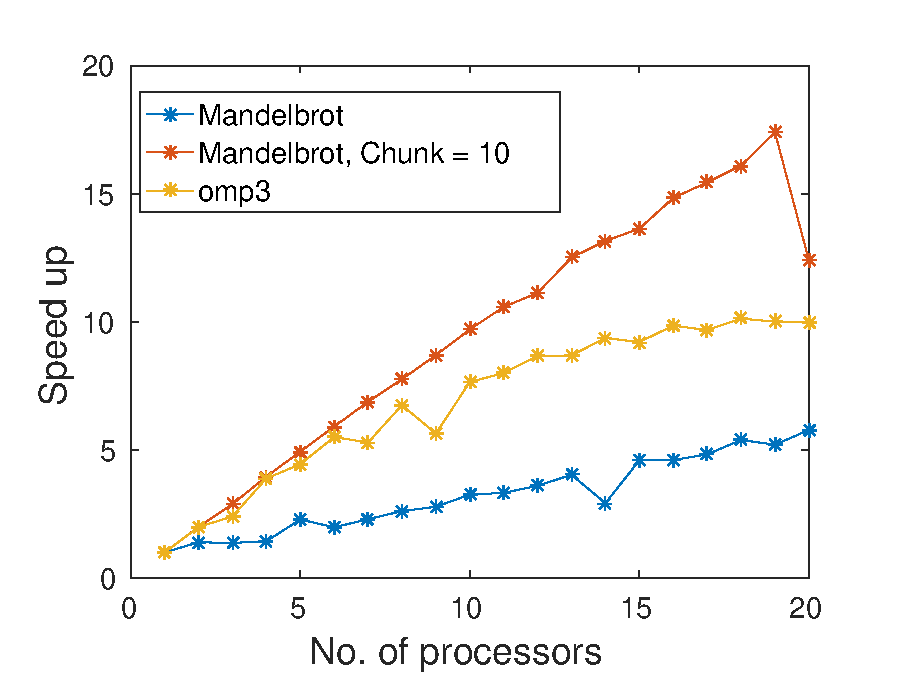
\includegraphics[width = 0.8\textwidth]{fig/mandelbrot.eps}
\caption{The speedup of the two the parallelization of the mandelbrot computation with the default scheduling, with a chunk size of 10 compared to the speedup of the Jacobi iteration.}
\label{fig:mandelbrot}
\end{figure}
